\documentclass{beamer}
\usetheme{IMM}

\usepackage{pgf,pgfarrows,pgfnodes,pgfautomata,pgfheaps,pgfshade}
\usepackage{amsmath,amssymb}
\usepackage[utf8]{inputenc}
\usepackage{colortbl}
\usepackage[english]{babel}
\usepackage{booktabs}
\usepackage{slpython}
\usepackage{underscore}
\usepackage{bm}

\author{Luis Pedro Coelho}
\institute{Programming for Scientists}

\graphicspath{{../figures/}{../figures/generated/}{../images/}}

\newcommand*{\code}[1]{\textsl{#1}}
\newcommand*{\Reals}[1]{R}
\newcommand*{\Assign}{\ensuremath{\leftarrow}}
\newcommand{\creditto}[1]{%
\begin{flushright}
(#1)
\end{flushright}%
}

\title{Homework/Review}
\usepackage{pgfpages}
\setbeameroption{show notes}
\setbeameroption{show notes on second screen}

\begin{document}
\frame{\maketitle}

\begin{frame}[fragile]
\frametitle{Homework}
\begin{itemize}
\item Download file
\item Open/parse it
\item Analyse it
\end{itemize}
\end{frame}

\begin{frame}[fragile]
\frametitle{FastQ Format}
According to Wikipedia, we get a sequence every four lines:

\begin{enumerate}
\item Header
\item DNA sequence
\item $+$ line
\item Qualities
\end{enumerate}

\begin{python}
ifile = open('hw-HeLa.fq')
while True:
    header = ifile.readline().strip()
    seq = ifile.readline().strip()
    _ = ifile.readline().strip()
    qualities = ifile.readline().strip()
    if not len(qualities):
        break
\end{python}

(This is not the only way to structure this)
\end{frame}

\begin{frame}[fragile]
\frametitle{Converting Qualities}
\begin{itemize}
\item We have read it as a string
\item We have a sequence of characters
\item Now, we want to get the numeric value
\end{itemize}

We will look it up.
\end{frame}

\begin{frame}[fragile]
\frametitle{Continuing}

\begin{python}
import numpy as np
. . .
while True:
    . . .
    qualities = [(ord(q) - 64) for q in qualities]
    qualities = np.array(qualities)
\end{python}

\end{frame}


\begin{frame}[fragile]
\frametitle{Let us compute the averages}

\begin{python}
import numpy as np
from matplotlib import pyplot as plt

allqs = []
ifile = open('hw-HeLa.fq')
while True:
    header = ifile.readline().strip()
    seq = ifile.readline().strip()
    _ = ifile.readline().strip()
    qualities = ifile.readline().strip()
    if not len(qualities):
        break
    qualities = [(ord(q) - 64) for q in qualities]
    qualities = np.array(qualities)
    allqs.append(qualities)
allqs = np.array(allqs)
\end{python}
\end{frame}

\begin{frame}[fragile]
\frametitle{Continuing\ldots}

Now we have an array named \lstinline{allqs} with all the qualities

\begin{python}
mean = allqs.mean(0)
std = allqs.std(0)
\end{python}

\pause

\begin{python}
gray = (.7,.7,.7)
plt.fill_between(
    np.arange(allqs.shape[1]),
    mean-std,
    mean+std,
    color=gray)
plt.plot(mean, color='k', lw=4)
plt.show()
\end{python}

\end{frame}


\begin{frame}[fragile]
\frametitle{Output}

\centering
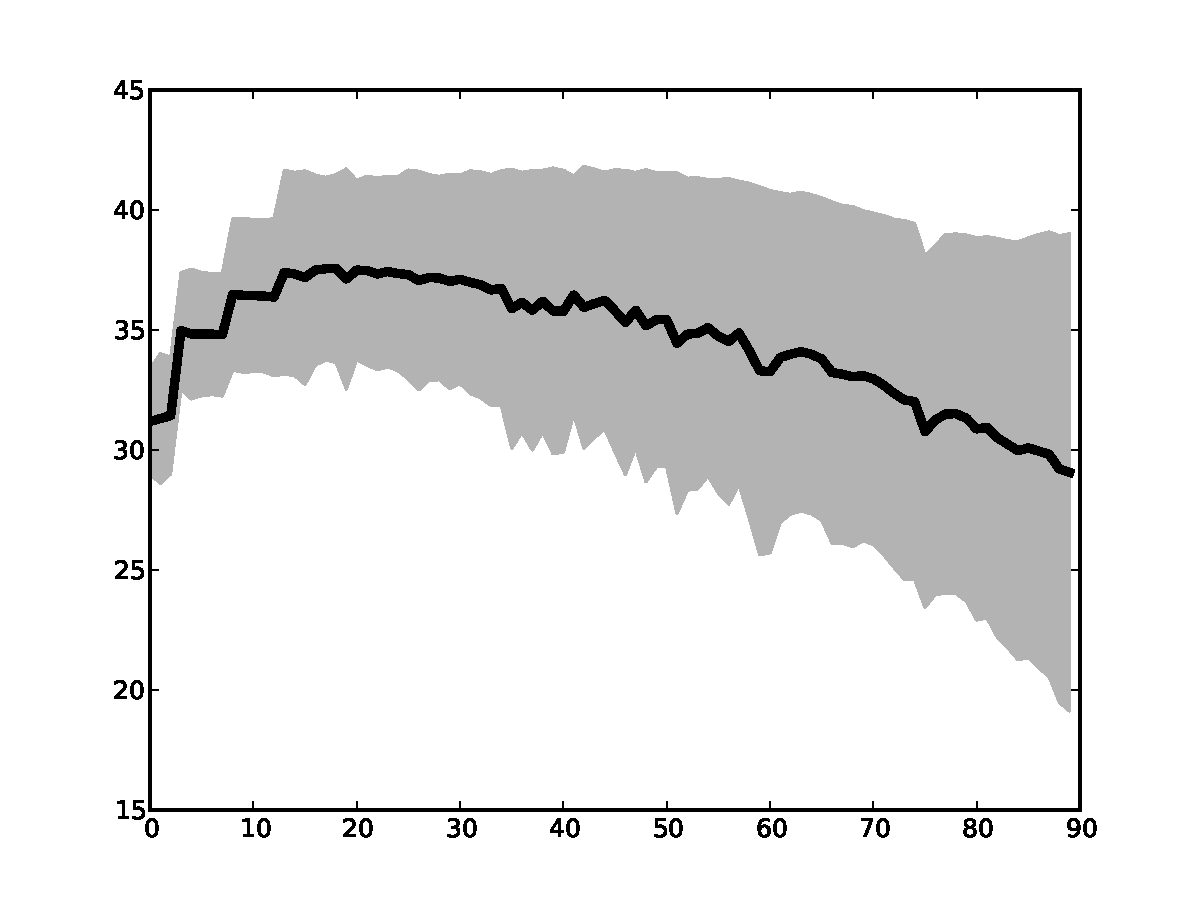
\includegraphics[width=.7\textwidth]{qualities}

\end{frame}

\begin{frame}[fragile]
\frametitle{Minor Improvements}

\begin{itemize}
\item So far, as I said, I used the file after unzipping
\item Can we use the file \alert{as is}?
\item For that, we need to open a gzipped file.
\item Let us look it up\ldots
\end{itemize}

\end{frame}

\begin{frame}[fragile]
\frametitle{gzip Module}


Replace

\begin{python}
ifile = open('hw-HeLa.fq')
\end{python}

by

\begin{python}
import gzip
ifile = gzip.open('hw-HeLa.fq.gz')
\end{python}
\end{frame}

\note{break}

\begin{frame}[fragile]
\frametitle{Trimming}

\centering
\includegraphics[width=.7\textwidth]{fastqtrim}

\end{frame}

\begin{frame}[fragile]
\frametitle{Algorithm}

\begin{enumerate}
\item We look from left to right.
\item Remember the longest substring we have seen.
\item When we are done, the longest substring will be it.
\end{enumerate}

\end{frame}

\begin{frame}[fragile]
\frametitle{Code}
\begin{python}
def trim(qs, thresh):
    bestlen = 0
    startcur = 0
    for i in xrange(len(qs)+1):
        if i >= len(qs) or qs[i] < thresh:
            curlen = i - startcur
            if curlen > bestlen:
                bestlen = curlen
                best = (startcur,i)
            startcur = (i+1)
    s,e = best
    return s,e
\end{python}
\end{frame}

\begin{frame}[fragile]
\frametitle{Putting it Together}

Let us look at the source code\ldots
\end{frame}

\begin{frame}[fragile]
\frametitle{Improvements}
\begin{itemize}
\item Do it in one pass
\end{itemize}
\end{frame}

\end{document}
